\providecommand{\toplevelprefix}{../..}  %
\documentclass[../../book-main.tex]{subfiles}

\begin{document}

\chapter{Future Study of Intelligence}
\label{ch:future}


  

\begin{quote}
``{\em The study is to proceed on the basis of the conjecture that every aspect of learning or any other feature of intelligence can in principle be so precisely described that a machine can be made to simulate it. An attempt will be made to find how to make machines use language, form abstractions and concepts, solve kinds of problem now reserved for humans, and improve themselves.}''

$~$\hfill -- Proposal for the Dartmouth AI program, 1956
 \end{quote}
\vspace{5mm}


This manuscript systematically introduces mathematical principles and computational mechanisms for how memory or knowledge can be developed from empirical observations. The ability to seek parsimony in a seemingly random world is a fundamental characteristic of any intelligence, natural or man-made. We believe the principles and mechanisms presented in this book are unifying and universal, applicable to both animals and machines.

We hope this book helps readers fully clarify the mystery surrounding modern practices of artificial deep neural networks by developing a rigorous understanding of their functions and roles in learning low-dimensional distributions from high-dimensional data. With this understanding, the capabilities and limitations of existing AI models and systems become clear:
\begin{enumerate}
    \item Existing models and systems fall short of being complete memory systems capable of self-learning and self-improving.
    \item Existing realizations of these functions remain primitive and brute-force, far from optimal in terms of optimization strategies and network architectures.
    \item Existing AI models only learn data distributions and conduct inductive (Bayesian) inference, which differs from high-level human intelligence.
\end{enumerate}

One goal of this book is to help readers establish an objective and systematic understanding of current machine intelligence technologies and to recognize what open problems and challenges remain for further advancement of machine intelligence. In the last chapter, we provide some of our views and projections for the future.

\section{Towards Autonomous Intelligence: Close the Loop?}
From the practice of machine intelligence in the past decade, it has become clear that, given sufficient data and computational resources, one can build a large enough model and pre-train it to learn the \textit{prior} distribution of all the data, say \(p(\vx)\). Theoretically, such a large model can memorize almost all existing knowledge about the world that has been encoded in text and images. As we discussed at the beginning of the book, such a large model plays a role similar to DNA, which life uses to record and pass on knowledge about the world.

The model and distribution learned in this way can then be used to create new data samples drawn from the same distribution. One can also use the model to conduct inference (e.g., completion, estimation, and prediction) with the memorized knowledge under various conditions, say by sampling the \textit{posterior} distribution \(p(\vx\mid \vy)\) under a new observation \(\vy\). Strictly speaking, such inference is statistical.

Any pre-trained model, however large, cannot guarantee that the distribution it has learned so far is entirely correct or complete. If our samples \(\hat{\vx}_{t}\) from the current \textit{prior} \(p_{t}(\vx)\) or estimates \(\hat{\vx}_{t}(\vy)\) based on the \textit{posterior} \(p_{t}(\vx\mid \vy)\) are inconsistent with the truth \(\vx\), we would like to correct the learned distributions:
\begin{equation}
    p_{t}(\vx) \rightarrow p_{t+1}(\vx) \quad \text{or}\quad p_{t}(\vx\mid \vy) \rightarrow p_{t+1}(\vx\mid \vy),
\end{equation}
based on the error \(\ve_{t} = \vx_{t} - \hat{\vx}_{t}\). This is known as error correction based on error feedback, a ubiquitous mechanism in nature for continuous learning. However, any open-ended model itself lacks the mechanism to revise or improve the learned distribution when it is incorrect or incomplete. Improving current AI models still depends largely on human involvement: supervision or reinforcement through experimentation, evaluation, and selection. We may call this process ``artificial selection'' of large models, as opposed to the natural selection for the evolution of life.

As we studied earlier in this book (\Cref{ch:closed-loop} in particular), closed-loop systems align an internal representation with sensed observations of the external world. They can continuously improve the internally learned distribution and its representation to achieve consistency or self-consistency. An immediate next step is to develop truly closed-loop memory systems, illustrated in \Cref{fig:open-to-closed}, that autonomously and continuously learn general data distributions and improve based on error feedback.

Therefore, the transition from the currently popular end-to-end trained open-loop models to continuously learning closed-loop systems
\begin{equation}
   \text{\textbf{open-ended} models} \; \Longrightarrow \; 
   \text{\textbf{closed-loop} systems}
\end{equation}
is the key for machines to truly emulate how the animal brain learns and applies knowledge in an open world. We believe that
\begin{quote}
\begin{center}
        \textit{open-ended models are for a closed world, however large; \\ closed-loop systems are for an open world, however small.}
\end{center}
\end{quote}
In fact, ``general intelligence'' can never be achieved by simply memorizing all existing data and knowledge of the world. Instead, general intelligence requires mechanisms to improve existing memory so as to adapt to new environments and tasks. This is precisely the essence of the Cybernetics program laid out by Norbert Wiener in the 1940s that we discussed at the very beginning of this book.

\begin{figure}[t]
    \centering    
    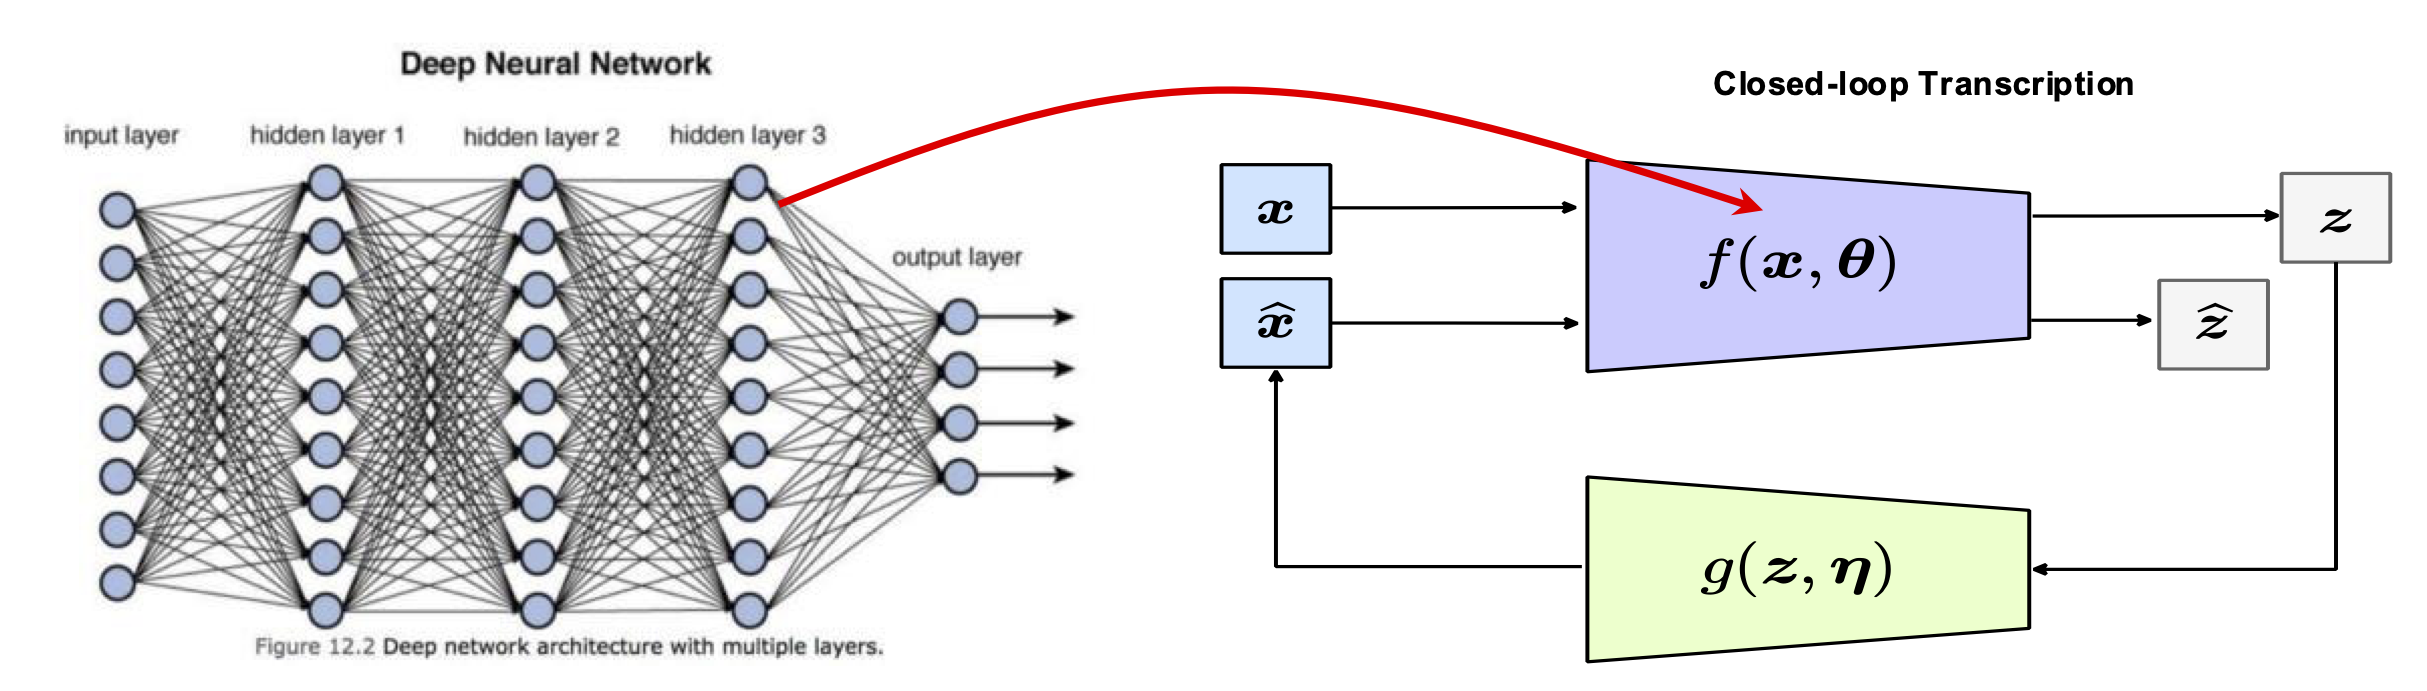
\includegraphics[width=0.9\linewidth]{\toplevelprefix/chapters/chapter8/figs/open-to-closed.png}
    \caption{From an open-ended deep network to a closed-loop system.}
    \label{fig:open-to-closed}
\end{figure}



\section{Towards the Intelligence of Nature: Beyond Back Propagation?}
The practice of machine intelligence in recent years has led many to believe that one must build a single large model to learn the distribution of all data and memorize all knowledge. Even though this is technologically possible, such a solution is likely far from necessary or efficient. As we know from training deep networks, the only known scalable method to train such networks at scale is through back propagation (BP) \cite{Back-Prop}. Although BP offers a way to correct errors via gradient signals propagated back through the whole model, it is nevertheless rather brute-force and differs significantly from how nature learns: BP is an option that nature cannot afford due to its high cost and simply cannot implement due to physical limitations.

More generally, we cannot truly understand intelligence unless we also understand how it can be efficiently implemented. That is, one needs to address the computational complexity of realizing mechanisms associated with achieving the objectives of intelligence. Historically, our understanding of (machine) intelligence has evolved through several phases, from the incomputable Kolmogorov complexity to Shannon's entropy, from Turing's computability to later understanding of tractability,\footnote{We say a problem is tractable if it allows an algorithm whose complexity is polynomial in the size of the problem.} and to the strong emphasis on algorithm scalability in modern practice of high-dimensional data analysis \cite{Wright-Ma-2022} and artificial intelligence. This evolution can be summarized as follows:
\begin{equation}
   \text{\textbf{incomputable}} \;
   \Longrightarrow \; \text{\textbf{computable}} \;
   \Longrightarrow \; \text{\textbf{tractable}} \; \Longrightarrow \; 
   \text{\textbf{scalable}}.
\end{equation}
To a large extent, the success and popularity of deep learning and back propagation is precisely because they have offered a scalable implementation with modern computing platforms (such as GPUs) for processing and compressing massive data. Nevertheless, such an implementation is still far more expensive than how nature realizes intelligence.

There remains significant room to improve the efficiency of machine intelligence so that it can emulate the efficiency of natural intelligence, which should be orders of magnitude greater than current brute-force implementations. To this end, we need to discover new learning architectures and optimization mechanisms that enable learning data distributions under natural physical conditions and resource constraints, similar to those faced by intelligent beings in nature---for example, without accessing all data at once or updating all model parameters simultaneously (via BP).

The principled framework and approach laid out in this book can guide us to discover such new architectures and mechanisms. These new architectures and mechanisms should enable online continuous learning and should be updatable through highly localized and sparse forward or backward optimization.\footnote{For learning a distribution, a simple instantiation of these desiderata is in the simplest case of PCA, with the online PCA method introduced in \Cref{ch:autoencoding}. The easier task of learning an online predictive model does not necessarily require learning the data distribution, and can be accomplished by existing methods such as the Kalman filter, etc. \cite{peng2025mathematics}.}

\begin{figure}[t]
\centering
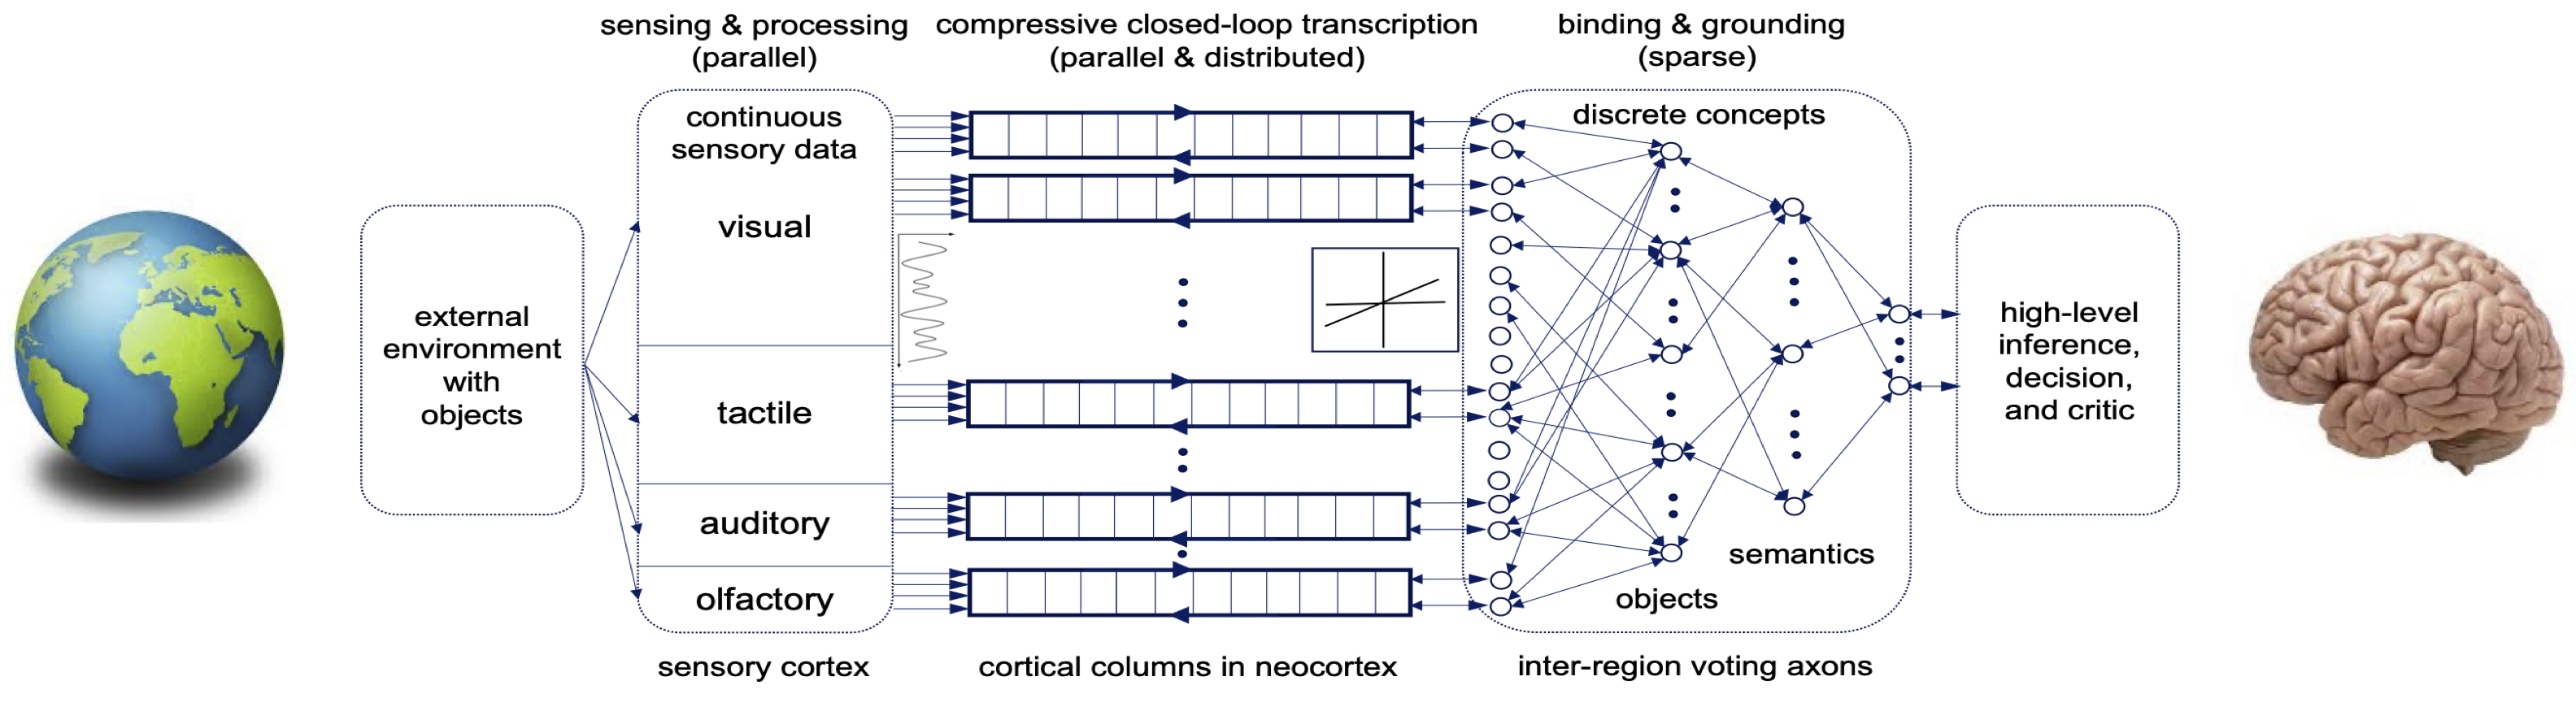
\includegraphics[width=0.99\linewidth]{\toplevelprefix/chapters/chapter8/figs/loops.png}
    \caption{Conjectured architecture of the brain cortex. The cortex is a massively parallel and distributed auto-encoding system consisting of a hierarchy of closed-loop auto-encoders that extract information from multiple senses and maximize the information gain of the resulting representations at multiple levels of hierarchy and granularity.}
    \label{fig:loops}
\end{figure}
As we have learned from neuroscience, the cortex of our brain consists of tens of thousands of cortical columns \cite{Hawkins-2021}. All cortical columns have similar physical structures and functions. They are highly parallel and distributed, though sparsely interconnected. Hence, we believe that to develop a more scalable and structured memory system, we need to consider architectures that emulate those of the cortex. \Cref{fig:loops} shows such a hypothesized architecture: a massively distributed and hierarchical system consisting of many largely parallel closed-loop auto-encoding modules.\footnote{Elements of such hypothetical architectures exist in the literature in various forms, such as predictive coding networks \cite{millidge2022predictive}, which have an optimization strategy that utilizes efficient local updates.} These modules learn to encode different sensory modalities or many projections of data from each sensory modality. Our discussion in \Cref{sec:measurement-self-consistency} of \Cref{ch:conditional-inference} suggests that such parallel sensing and learning of a low-dimensional distribution is theoretically possible. Higher-level (lossy) autoencoders can then be learned based on outputs of lower-level ones to develop more sparse and higher-level ``abstractions'' of the representations learned by the lower levels.

The distributed, hierarchical, and closed-loop system architecture illustrated in \Cref{fig:loops} shares many characteristics of the brain's cortex. Such a system architecture may open up many more possibilities than the current single large-model architecture. It enables exploration of much more efficient learning and optimization mechanisms and results in a more structured modular organization of the learned data distribution and knowledge. This would allow us to bring the implementation of machine intelligence to the next level of evolution:
\begin{equation}
   \text{\textbf{incomputable}} \;
   \Longrightarrow \; \text{\textbf{computable}} \;
   \Longrightarrow \; \text{\textbf{tractable}} \; \Longrightarrow \; 
   \text{\textbf{scalable}} \; \Longrightarrow \; 
   \text{\textbf{natural}}.
\end{equation}

\section{Towards the Scientific Intelligence of Humans: Beyond the Turing Test?}
As we have discussed at the beginning of this book, \Cref{ch:intro}, intelligence in nature has evolved through multiple phases and manifested in four different forms:
\begin{equation}
    \text{\textbf{phylogenetic}} \;
    \Longrightarrow \; \text{\textbf{ontogenetic}} \; 
    \Longrightarrow \; \text{\textbf{societal}} \; 
    \Longrightarrow \; \text{\textbf{scientific intelligence}}.
\end{equation}
All forms of intelligence share the common objective of learning useful knowledge as low-dimensional distributions of sensed high-dimensional data about the world. However, they differ significantly in the specific coding schemes adopted, the information encoded, the computational mechanisms for learning and improving, and the physical implementations of such mechanisms. Using the concepts and terminology developed in this book, the four stages of intelligence differ in the following three aspects:
\begin{enumerate}
    \item The \textit{codebook} used to learn and encode the intended information or knowledge.
    \item The \textit{information} or knowledge encoded and represented using the codebook. 
    \item The \textit{optimization mechanisms} used to improve the encoded information or knowledge.
\end{enumerate}
The following table summarizes their main characteristics:
\begin{table}[h]
    \centering
    \begin{tabular}{| c | c | c | c | c |}
    \hline & \textbf{Phylogenetic} & \textbf{Ontogenetic} & \textbf{Societal} & \textbf{Scientific}\\
    \hline
    \textbf{Codebook}  & Amino Acids & Neurons & Alphabet \& Words & Mathematics/Logic \\ [0.5ex]
    \hline 
    \textbf{Information} & Genes/DNAs & Memory & Languages/Texts & Scientific Facts\\ [0.5ex]
    \hline
    \textbf{Optimization} & Genetic Selection & Error Feedback & Trial \& Error & Hypothesis Testing \\  [0.5ex]
    \hline
    \end{tabular}
    \caption{Main characteristics of the four stages of intelligence.}    
\end{table}


As we now know, humans have achieved two quantum leaps in intelligence. The first was the development of spoken and written language, which enabled humans to share and transmit learned knowledge across generations, much as DNA does in nature. The second was the development of mathematics and formal logic roughly three thousand years ago, which became the precise language of modern science. This new language freed us from summarizing knowledge from observations in empirical form and allowed us to formalize knowledge as verifiable theories falsifiable through mathematical deduction or experimental verification. Through hypothesis formulation, logical deduction, and experimental testing, we can now proactively discover and develop new knowledge that was previously impossible by passively learning from observed data distributions.\footnote{For example, causal relationships cannot be learned from distributions alone \cite{Pearl-2009}.}

As discussed in the introduction (\Cref{ch:intro}), the 1956 ``artificial intelligence'' (AI) program aimed precisely to study how to endow machines with scientific intelligence, i.e., high-level functions such as mathematical abstraction, logical inference, and problem solving that are believed to differentiate humans from animals:
\begin{equation}
   \text{\textbf{low-level} (animal) intelligence} \; \Longrightarrow \; 
   \text{\textbf{high-level} (human) intelligence.}
\end{equation}
As we have clarified repeatedly in this book, most technological advances in machine intelligence over the past decades, although carried out under the name ``AI'', are actually more closely related to the low-level intelligence shared by both animals and humans, which is mainly inductive. So far, no evidence suggests that these mechanisms alone suffice to achieve the high-level human intelligence that the original AI program truly aimed to understand and emulate.

% Start of Selection
In fact, we know little about how to rigorously verify whether a system is truly capable of high-level intelligence, even though the Turing test was proposed in 1950 \cite{Turing-1950}.\footnote{In Turing's proposal, the evaluator is a human. However, most human evaluators have limited scientific training and knowledge, and their conclusions can be subjective.} For a long time, such a test was not deemed necessary since machine capabilities were far below those of humans (or even animals). However, given recent technological advances, many models and systems now claim to reach or even surpass human intelligence. Therefore, it is high time to develop a scientific and executable definition of the Turing test, i.e., a systematic and objective method to evaluate the intelligence level of a given model or system. For example, how can we rigorously verify whether an intelligent system has truly grasped an abstract concept such as the natural or real numbers, or whether it has merely memorized numerous instances? Note that state-of-the-art large language models still struggle with simple mathematical questions like: ``Is 3.11 larger or smaller than 3.9?''\footnote{Some models have corrected their answers to such questions through targeted engineering, or have incorporated additional reasoning mechanisms that verify immediate answers and correct them during reasoning. However, we leave it to the reader as an exercise to rigorously test whether any state-of-the-art language model truly understands the notion of numbers (natural, rational, real, and complex) and their associated arithmetic.}

How do we verify whether a system truly understands the rules of logic and can apply them rigorously, or has merely memorized a large number of logical instances? Furthermore, is such a system capable of correcting its own knowledge or developing new knowledge, such as physical laws, mathematical concepts, or causal relationships? In summary, it is high time we develop rigorous evaluation methods to determine which of the following categories a system's seemingly intelligent capability belongs to:
\begin{enumerate}
    \item having merely memorized the distribution of some knowledge-carrying data and regenerating it;
    \item being able to autonomously and continuously develop new knowledge from new observations;
    \item having truly understood certain abstract knowledge and knowing how to apply it correctly;
    \item being able to generate new scientific hypotheses or mathematical conjectures and verify them.
\end{enumerate}

\begin{figure}[t]
    \centering
    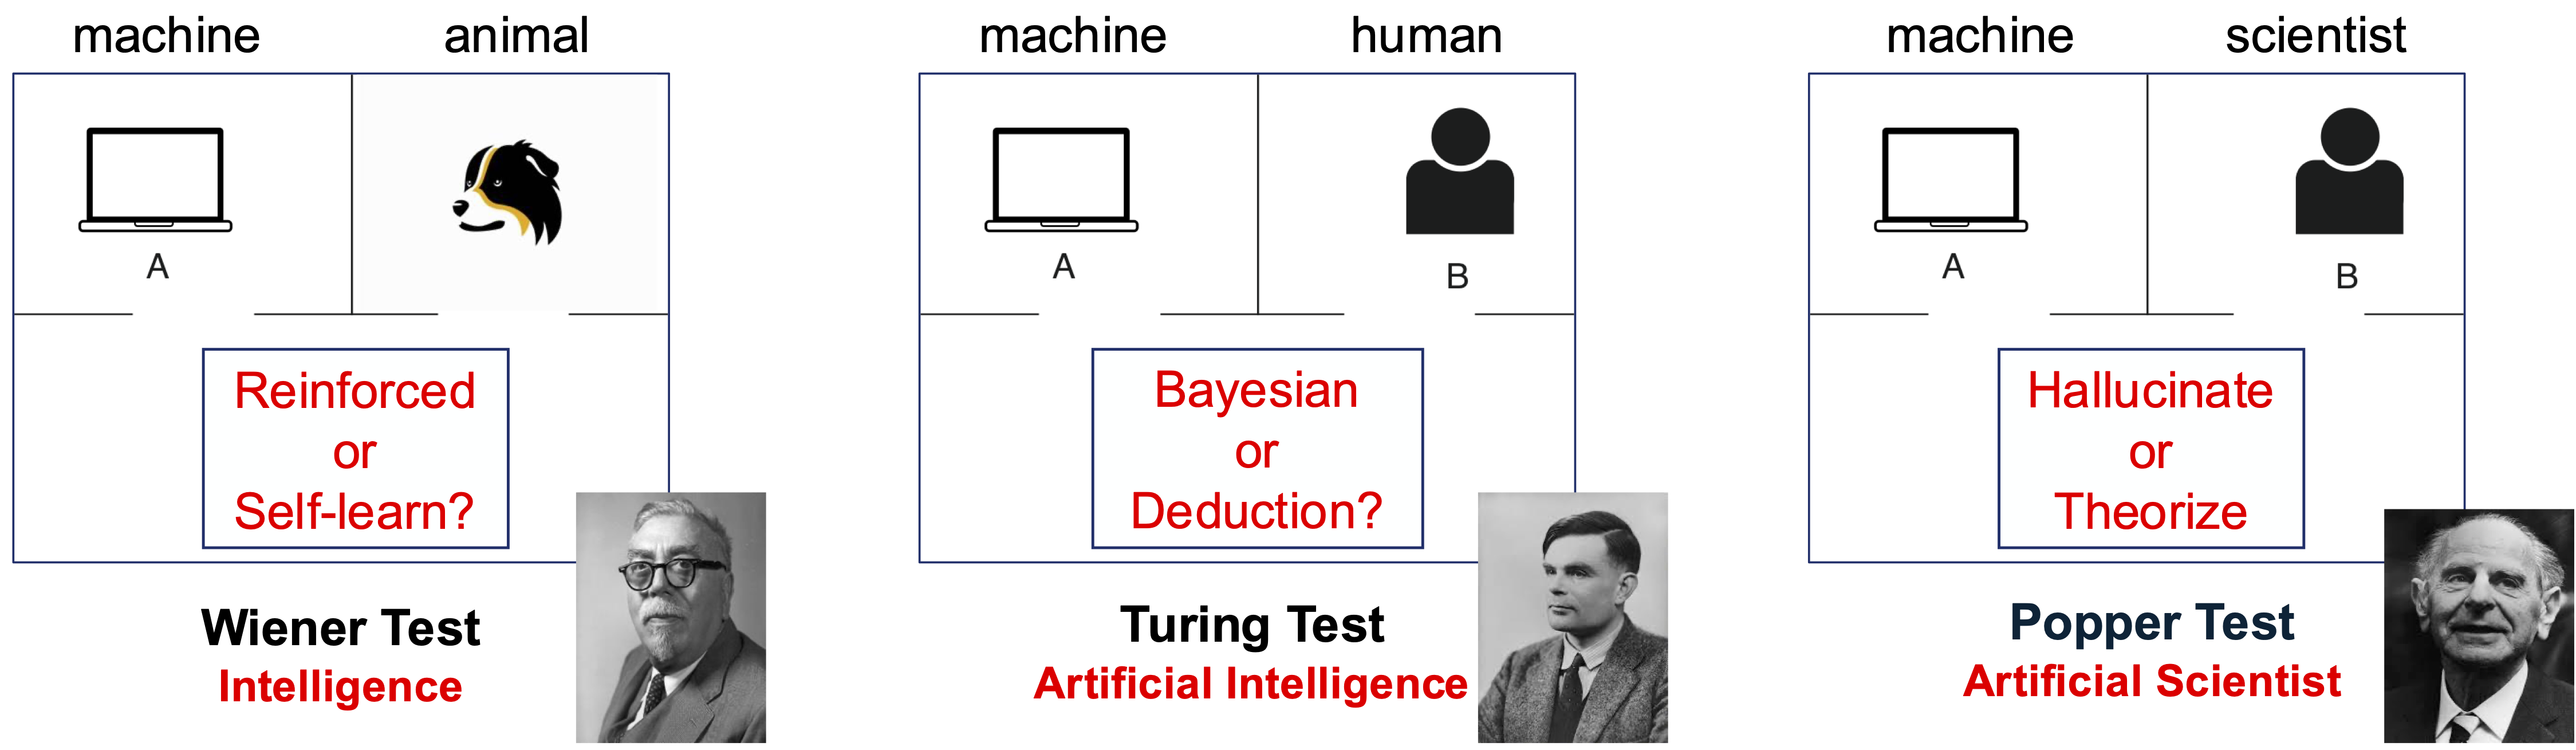
\includegraphics[width=0.95\linewidth]{\toplevelprefix/chapters/chapter8/figs/tests.png}
    \caption{Three tests for different levels or types of intelligence capabilities: the Wiener test for basic intelligence, the Turing test for human-level intelligence, and the Popper test for scientist-level intelligence.}
    \label{fig:three-tests}
\end{figure}

\Cref{fig:three-tests} illustrates that there should probably be at least three different tests to evaluate and distinguish among types of intelligence:
\begin{enumerate}
    \item \textit{The Norbert Wiener test:} to determine whether a system can improve and develop new knowledge on its own or merely receives information through reinforcement or supervised learning;
    \item \textit{The Alan Turing test:} to determine whether a system understands abstract knowledge or merely learns its statistics and uses them for Bayesian inference;
    \item \textit{The Karl Popper test:} to determine whether a system can explore new knowledge by forming and verifying theories based on self-consistency.
\end{enumerate}
We believe that, for such evaluations, the evaluator should not be a human but rather a scientifically sound protocol and process.

As we have seen throughout this book, \textit{compression} has played a fundamental role in learning. It is the governing principle and a unified mechanism for identifying an empirical data distribution and organizing the information encoded therein. To a large extent, it explains most of the practice of ``artificial intelligence'' in the past decade. An outstanding question for future study is whether \textit{compression alone} is sufficient to achieve all the higher-level capabilities of intelligence listed above. 
\begin{quote}
    \centering
    \textit{Is compression all there is?}
\end{quote}
Are abstraction, causal inference, logical reasoning, hypothesis generation, and deduction extended or extreme forms of compression? Is there a fundamental difference between identifying empirical data distributions through compression and forming high-level abstract concepts and theories? Philosopher Sir Karl Popper once suggested:
\begin{quote}
    \centering
    \textit{``Science may be described as the art of systematic oversimplification.''}
\end{quote}
To a large extent, science---and its associated codebook, mathematics---can be viewed as the most abstract form of intelligence, unique to educated and enlightened humans, akin to a form of high art. We believe that uncovering and understanding the underlying mathematical principles and computational mechanisms of such higher-level intelligence will be the final frontier for science, mathematics, and computation altogether!

\end{document}
